This comprises an outer ellipse with semi-axes $(a,b)$ and an internal circle of radius $r$, Figure~\ref{fig:inner-circle}.

\begin{figure}
    \centering
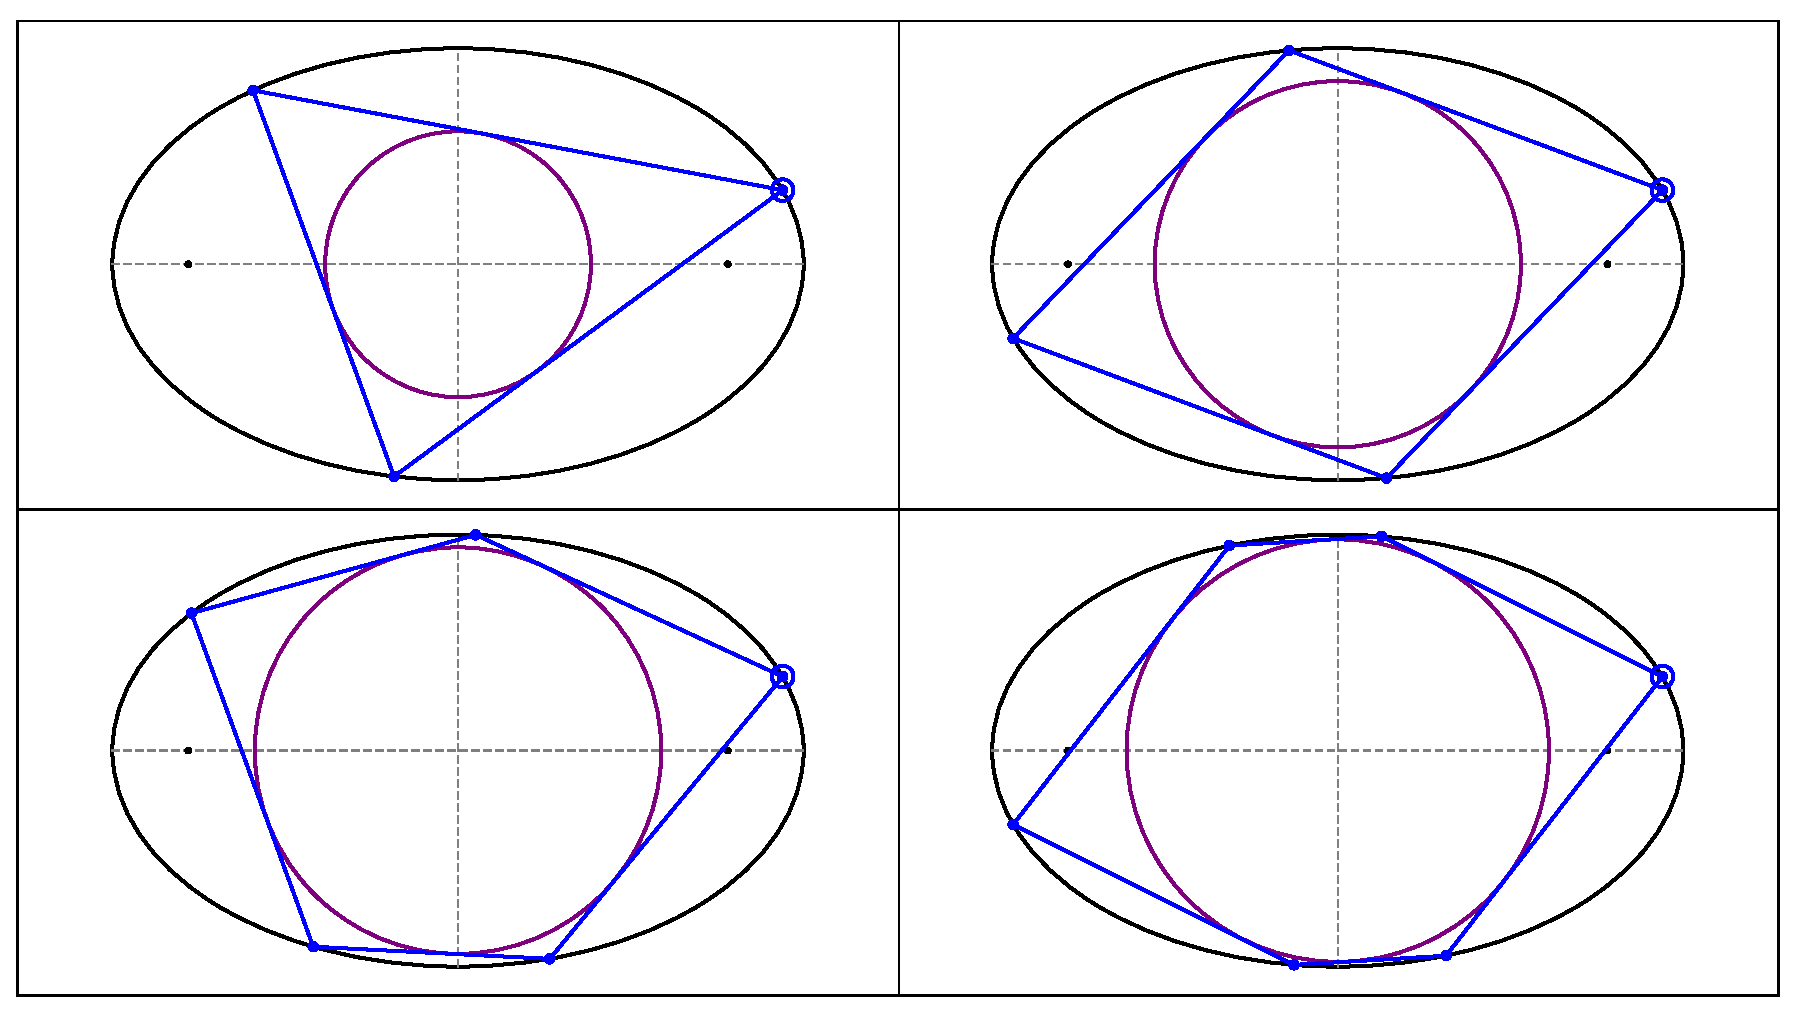
\includegraphics[width=\textwidth]{pics/0010_system_I.eps}
    \caption{System I pair comprising an external ellipse and an internal circle. Shown are N-periodics for $N=3,4,5,6$.}
    \label{fig:inner-circle}
\end{figure}

For the $N=3$ case the internal circle becomes the (stationary) incircle with fixed inradius $r$, and from \eqref{eqn:pair-n3} obtain:

\[ r=\frac{{a}{b}}{a+b}\]

\noindent Referring to Figure~\ref{fig:ellipse-circle-poristic} (left):

\begin{proposition}
The family of System I 3-periodics has invariant circumradius $R=(a+b)/2$. Furthermore, the locus of the circumcenter $X_3$ is a circle of radius $d=R-b=a-R$ about $O=X_1$.
\label{prop:R}
\end{proposition}

\begin{proof}
Consider the explicit expressions derived for 3-periodic vertices in Appendix~\ref{app:explicit-I}. From this obtain that the circumcircle of the orbit has center 
	\[X_3=\left[ - \,{\frac {x_1\, \left( a-b \right)  \left( -x_1^{2}
			\left( a+b \right) ^{2}+{a}^{2}b \left( 2\,a+b \right)  \right) }{2a
			\left(  \left( {a}^{2}-{b}^{2} \right) x_1^{2}+{a}^{2}{b}^{2}
			\right) }}
	 ,  {\frac { \left( a-b \right)  \left( x_1^{2} \left( a+b
	 		\right) ^{2}-{a}^{2}{b}^{2} \right) y_1}{2b \left( {a}^{2}x_1^2+{b}^{2} \left( {a}^{2}-x_1^{2} \right)  \right) }}
	   \right]\]
	and radius $(a+b)/2$. Also obtain that the locus of $X_3$ is a circle with center $(0,0)$ and radius $(a-b)/2$.
	

\end{proof}
\begin{proposition} The power of origin with respect to the circumcircle is invariant and  equal to $-ab$
	
	
\end{proposition}


\begin{proof}
	\textcolor{red}{ronaldo}
	
\end{proof}

Recall the Poristic family of triangles with fixed, non-concentric incircle and circumcircle with centers separated by $d=\sqrt{R(R-2r)}$  \cite{gallatly1914-geometry,odehnal2011-poristic}. Let $\mathcal{I}$ be a (moving) reference frame centered on $X_1$ with one axis oriented toward $X_3$. Referring to Figure~\ref{fig:ellipse-circle-poristic} (right):

\begin{proposition}
With respect to $\mathcal{I}$, System I 3-periodics are the Poristic triangle family (modulo a rigid rotation about $X_1$).
\end{proposition}

\begin{proof}
This stems from the fact that $R$, $r$, and $d$ are constant. 
\end{proof}

As proved in \cite[Thm 3]{garcia2020-poristic}:

\begin{obs}
The $X_1$-centered circumconic to Poristics is a rigidly-rotating ellipse with axes $R+d$ and $R-d$.
\end{obs}

Since this circumellipse is identical (up to rotation) to System I's outer ellipse, so $R+d=a$ which is compatible with Proposition~\ref{prop:R}.

Furthermore, because poristic triangles are the image of Billiard 3-periodics under a (varying) affine transform \cite[Thm 4]{garcia2020-poristic}, it displays the same scale-free invariants.

\begin{corollary}
3-periodics in System I conserve the sum of cosines, product of half-sines, and all scale-free invariants.
\end{corollary}

\begin{figure}
    \centering
    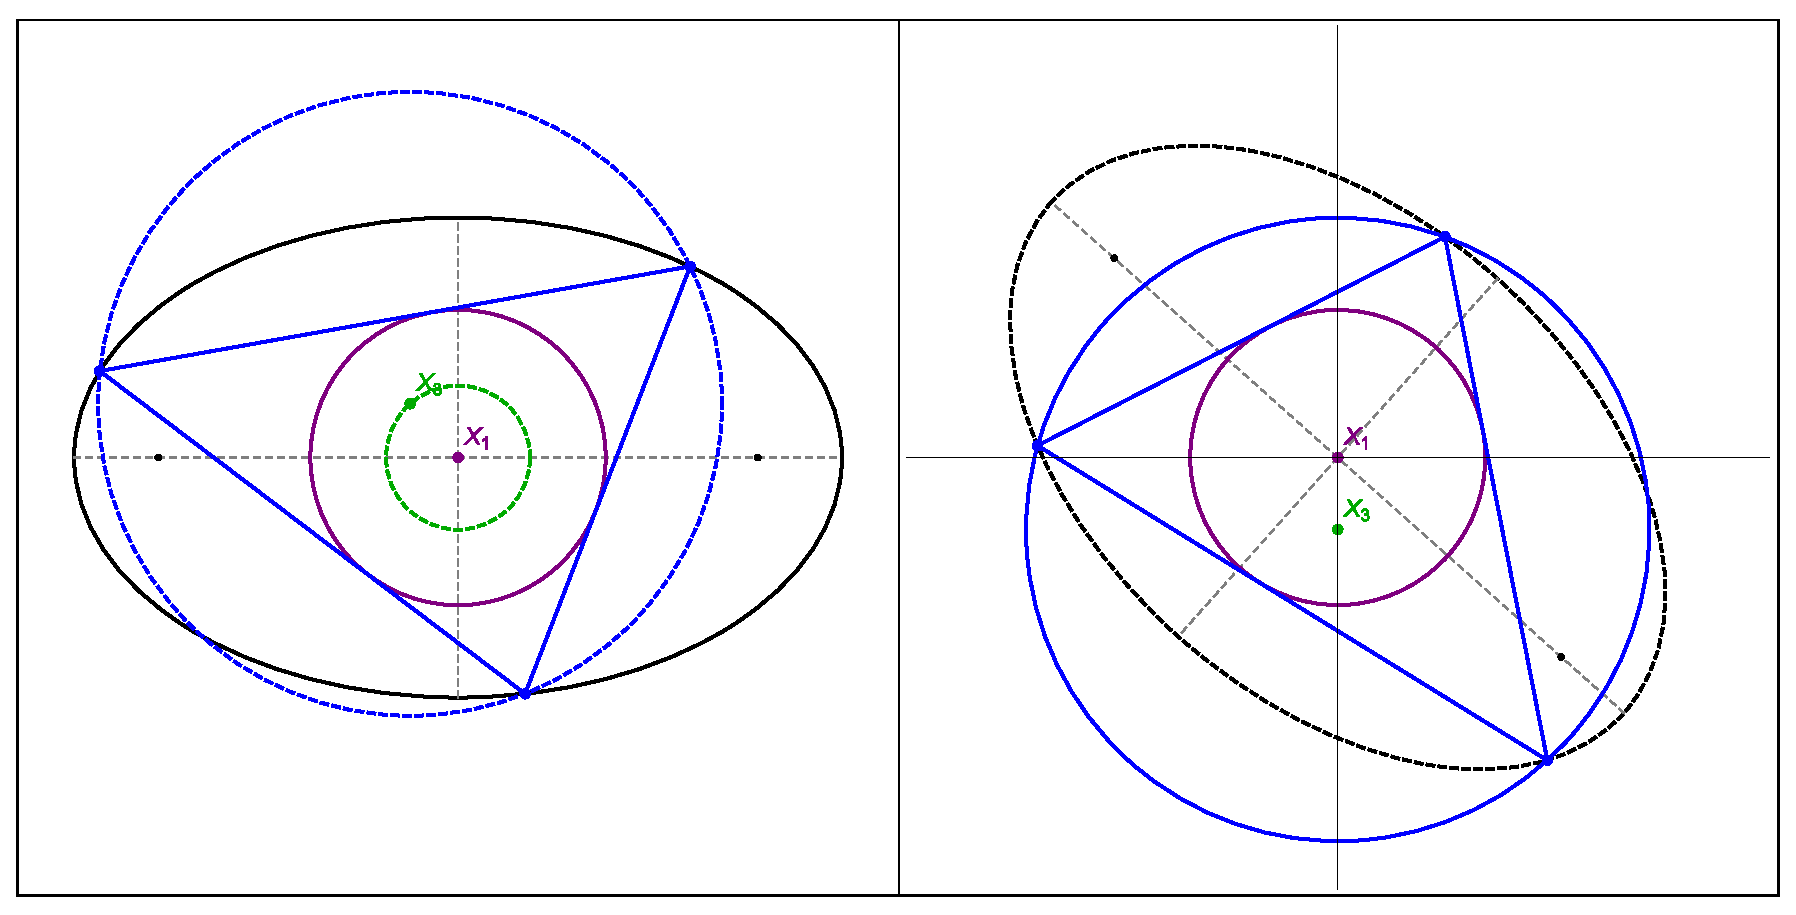
\includegraphics[width=\textwidth]{pics/0017_system_I_poristic.eps}
    \caption{System I 3-periodics (left) are identical (up to rotation) to the family of Poristic triangles (right) \cite{gallatly1914-geometry}, if the former is observed with respect to a reference system where $X_1$ and $X_3$ are fixed. The fixed incircle (resp. circumcircle) are shown purple (resp. blue). The original outer ellipse (black on both drawings) becomes the $X_1$-centered circumellipse in the Poristic case. Over the family, this ellipse is known to rigidly rotate about $X_1$ with axes $R+d,R-d$, where $d=|X_3-X_1|$ \cite{garcia2020-poristic}.}
    \label{fig:ellipse-circle-poristic}
\end{figure}

\subsection*{N>3}

Noting the barycentrics to the circumcenter $X_3$ are $\sin({2\theta_i})$ \cite{etc}. Since Steiner's {\em Curvature Centroid} $K$ is also the average of vertices weighted by $w_i=\sin({2\theta_i})$ \cite{steiner1838}, we will use it as an $N>3$ proxy for $X_3$. As depicted in Figure~\ref{fig:ellipse-circle-krummungs}:

\begin{conjecture}
For System I and an odd $N$, the locus of $K$ is an $O$-centered circle whose radius depends on $N$. If $N$ is even, $K$ is stationary at $O$.
\end{conjecture}

Let $A$ be the area of a System I N-periodic and $A_k$ be area of its pedal polygon with respect to $K$, whose vertices are the feet of perpendiculars dropped from $K$ onto the sides of the N-periodic, Figure~\ref{fig:ellipse-circle-krummungs}. Steiner proved such a polygon has extremal area \cite{steiner1838}. Suprisingly:

\begin{conjecture}
Given an odd $N$, the ratio $A_k/A$ for System I N-periodics is invariant over the family and only depends on $N$.
\end{conjecture}

\begin{figure}
    \centering
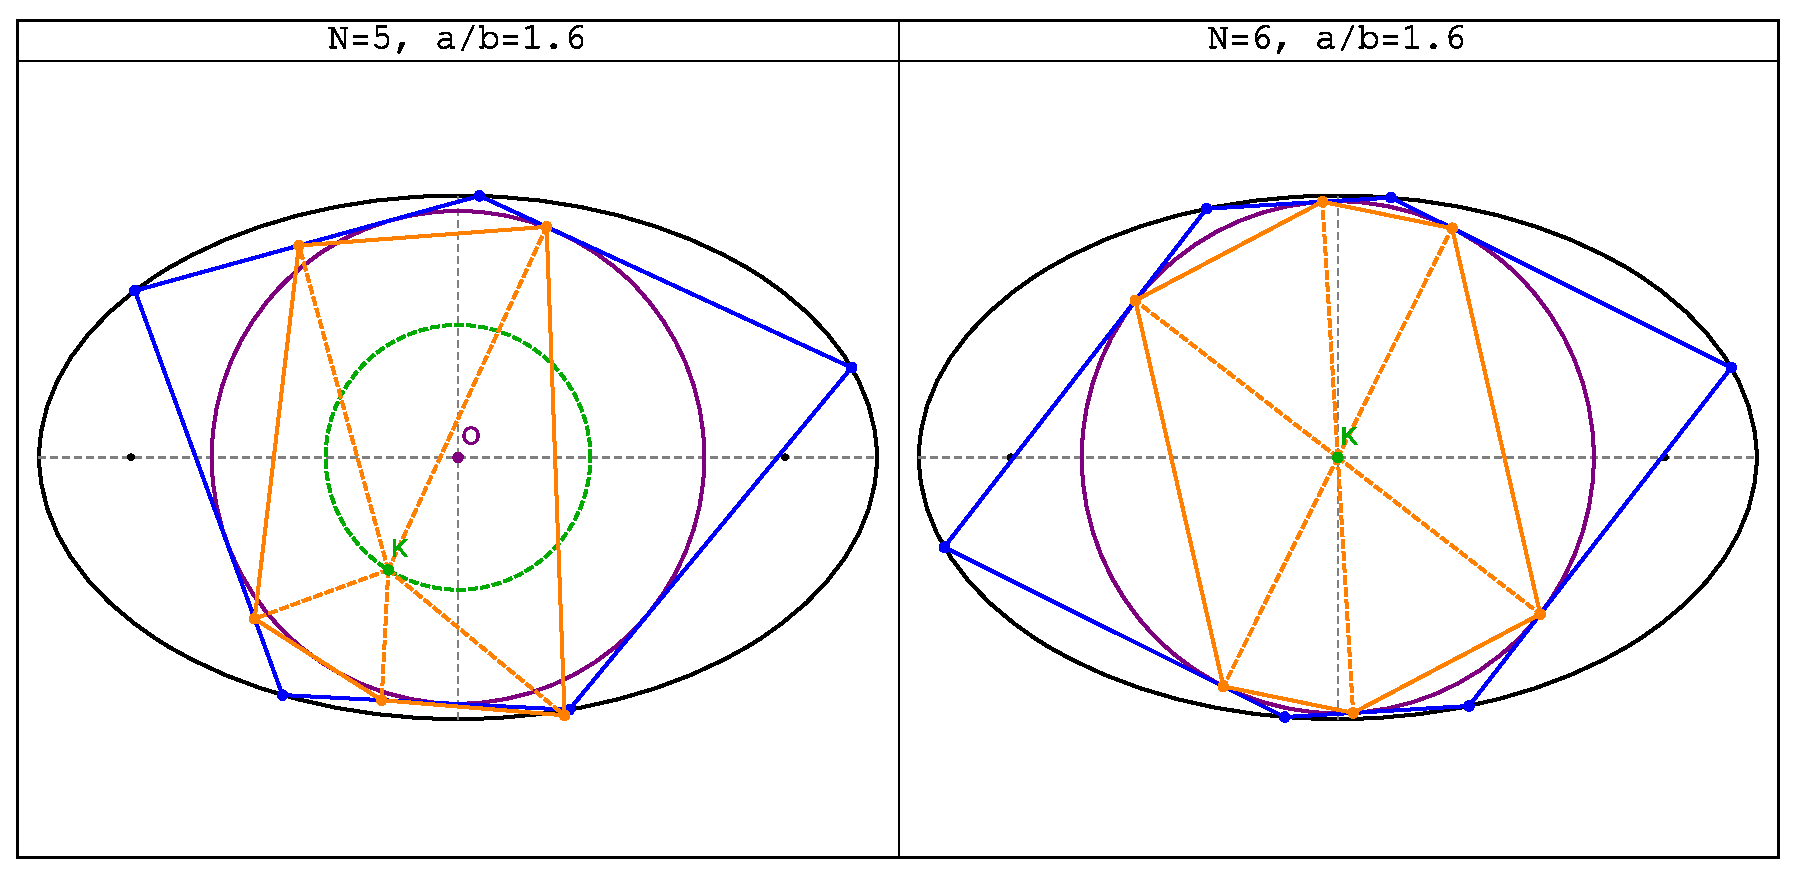
\includegraphics[width=\textwidth]{pics/0015_system_I_krummungs.eps}
    \caption{\textbf{Left}: System I at $N=6$: Steiner's Curvature Centroid $K$ moves along a circular locus (dashed green) centered on $O$. The pedal polygon to the 5-periodic with respect to $K$ (orange) has an area which is at an invariant ratio to that of the 5-periodic. \textbf{Right:} a System I  6-periodic is shown (blue). Because N is even $N$ is stationary at $O$ and the area ratio invariance no longer applies.}
    \label{fig:ellipse-circle-krummungs}
\end{figure}

For triangles, the following is a known relation \cite[Equation 3]{mw}:

\[ r R = \frac{\prod_{i=1}^3{s_i}}{2\sum_{i=1}^3{s_i}} \]

Since System I 3-periodics conserve both $R$ and $r$, the right-hand side of he above is invariant. Interestingly:

\begin{conjecture}
For System I odd N-periodics, the ratio of product-of-sidelengths to sum-of-sidelengths is invariant, i.e.:

\[ \frac{\prod_{i=1}^N{s_i}}{\sum_{i=1}^N{s_i}} = \text{invariant} \] 
\end{conjecture}

Referring to  \cite{reznik2020-forty} for a 40+ list of Elliptic Billiard N-periodic invariants:

\begin{conjecture}
N-Periodics in System I conserve all scale-free invariants displayed by System 0 N-Periodics, e.g., sum of cosines, product of half-sines (for odd N), etc.
\end{conjecture}
